\documentclass[12pt]{report}
\usepackage[top=23mm,bottom=23mm,left=23mm,right=23mm]{geometry}
\usepackage{fancyhdr, lastpage}
\usepackage{times}
\usepackage{cite}
\usepackage{chapterbib}
\usepackage[sectionbib]{natbib}
\bibpunct{(}{)}{;}{a}{,}{,}
\usepackage[pdftex]{graphicx}
\usepackage{epstopdf}
\usepackage{subfigure}
\usepackage[footnotesize, bf]{caption}
\usepackage{amsmath}
\usepackage{amssymb}
\usepackage{setspace}
\usepackage[small,compact]{titlesec}
\usepackage{multicol}
\usepackage{multirow}
\usepackage{wrapfig}
\usepackage{minitoc}
\usepackage{array}
\usepackage{tikz}
\usepackage{enumerate}  % for enumerating with a), b) etc...
\usepackage{caption}    % for having enumertion in a caption 
\usepackage{cleveref}   % So multiple references will auto format themself
\usepackage[]{algorithm2e}


%Folder paths that contain graphics
\graphicspath{{./}
{Chapters/ConvergenceFigures/}
{Chapters/IterationsFigures/}
{Chapters/MethodFigures/}
{Chapters/ModelFigures/}
{Chapters/Show1DFigures/}
{Chapters/Typical_SimulationFigures/}}


% PDF hyper-linking (set colors to black for printing)
%\usepackage[ps2pdf=true,colorlinks]{hyperref}
%\usepackage[figure,table]{hypcap}
%\hypersetup{
%	bookmarksnumbered,
%	pdfstartview={FitH},
%	citecolor={black},
%	linkcolor={black},
%	urlcolor={black},
%	pdfpagemode={UseOutlines}
%}

\pdfinfo{
/Author (Eric M. Jalbert, 2014)
/Title (Numerical Analysis of Methods for Simulating Clostridium Thermocellum)
/Subject (Numerical Analysis of Methods for Simulating Clostridium Thermocellum)
}

%Paragraph symmetries...
\setlength{\parskip}{10pt}
\setlength{\parindent}{0pt}
\setlength{\parsep}{0pt}


\setcounter{secnumdepth}{5}
\setcounter{tocdepth}{1}
\renewcommand{\mtctitle}{ }
\renewcommand{\mlftitle}{ List of Figures in Chapter }
\setcounter{minitocdepth}{1}
%\setcounter{minilofdepth}{2}
\renewcommand{\abstractname}{\Large ABSTRACT}
\renewcommand{\bibname}{References}
%\renewcommand\bibsection{}
%\renewcommand{\bibsep}{0pt}

\fancypagestyle{custom}{
\lhead{\textit{E.Jalbert, 2014}}
\rhead{\textit{NUMERICAL ANALYSIS SIMULATING C.THERMOCELLUM}}
}

\fancypagestyle{References}{
\lhead{}
\rhead{\textit{REFERENCES}}
}

%%%%%%%%% If I have appendies, add the fancy page styles 
%%%%%%%%% like the example below
%\fancypagestyle{AppendixA}{
%\lhead{}
%\rhead{\textit{APPENDIX A: Default Simulation Parameters}}
%}

\begin{document}

%PreliminarySections
\pagenumbering{roman}
%----------------------------------------------------------
% Title Page
%   The first page of the thesis, contains 
%   author/university/title and other info
%----------------------------------------------------------
\begin{titlepage}
  \begin{center}
    \vspace*{4cm}
    \LARGE\large{Comparison of a Semi-Implicit and a Fully-Implicit Time Integration Method for a Highly Degenerate Diffusion-Reaction Equation Coupled with an Ordinary Differential Equation}
    \vspace*{0.5cm}
    
    \small{by}
    \vspace*{0.5cm}
    
    \large{Eric M. Jalbert}
    \vspace*{3.5cm}
    
    A Thesis\\presented to\\The University of Guelph
    \vspace*{1.5cm}
    
    In partial fulfilment of requirements\\for the degree of\\Master of Science\\in\\Applied Mathematics
    \vfill

    Guelph, Ontario, Canada
    
    $\copyright$ E.M. Jalbert, January, 2015
  \end{center}
\end{titlepage}






%%Abstract
%\phantomsection
\addcontentsline{toc}{section}{Abstract}
%\section*{ABSTRACT}
\begin{abstract}
\setcounter{page}{2}
\begin{center}
%\vspace*{33pt}
\large{\textbf{Comparison of a Semi-Implicit and a Fully-Implicit Time Integration Method for a Highly Degenerate Diffusion-Reactor Equation Coupled with and Ordinary Differential Equation}}\\
\vspace*{20pt}
\begin{minipage}{0.49\textwidth}
\begin{flushleft}
\normalsize{Eric M. Jalbert}\\
\normalsize{University of Guelph,2015}
\end{flushleft}
\end{minipage}
\begin{minipage}{0.49\textwidth}
\begin{flushright}
\normalsize{Advisor}\\
\normalsize{Professor Hermann J. Eberl}
\end{flushright}
\end{minipage}
\end{center}
\vspace*{20pt}

%Degenerate diffusion-reaction equations tend to arise when modelling biofilm growth and propagations.
%Specifically focusing on \textit{Clostridium thermocellum}, because of its potential in the field of energy biotechnology, the model by \cite{dumitrache2015mathematicalModeling} is extended for spatial consideration.
%The resulting system is a partial differential equation coupled with an ordinary differential equation, these correspond to the diffusing biomass and the non-diffusing substrate.
%This introduces a degeneracy at the interface which makes typical numerical computations of the solution difficult.
%For this, a fully-implicit time integration method is formulated so that it generalises a semi-implicit method to solve the problem with addition accuracy.
%The fully-implicit method uses a fixed-point iteration and preselected tolerance to approximate the solutions at the next time step.
A certain class of highly degenerate diffusion equations arises when modelling biofilm growth and propagations.
We focus on the cellulolytic \textit{Clostridium thermocellum}, because of its potential in the field of energy biotechnology.
From this system a spatially implicit model was proposed in the literature before.
Here we study a spatially explicit model.
In contrast to other biofilm systems, a special feature of this system is that the growth promoting nutrient is not diffusive but bound in the substratum on which the biofilm grows.
As a consequence one obtains a highly degenerate diffusion-reaction equation for the bacteria that is coupled to an ordinary differential equation for nutrients.
The degeneracy of the biomass equation introduces gradient blow-up at the interface which makes numerical treatment difficult.
For this, a fully-implicit time integration method is formulated so that it generalises a previously used semi-implicit method to solve the problem with increased accuracy.
The fully-implicit method uses, at each time-step, a fixed-point iteration to solve the arising nonlinear algebraic equation and can be controlled by the required tolerance for convergence.

%The newly developed method is validated and tested to investigate numerous issues that arise with numerical computations: sinks or sources of biomass, loss of characteristics in the solution, and destruction of the conservation of mass.
%Once the certainty of the solutions for the fully-implicit method are confirmed, the difference between the fully-implicit and semi-implicit methods is quantified by use of quantitative measurements so that the benefits of the new method can be recorded.
%These measurement are called the normed differences, they are the $L_1$-norm and $L_2$-norm of the relative difference between the solutions. 
%The trade-off between improved accuracy and increased computational effort is determined to be optimal for tolerances that force a single extra iteration of the fully-implicit method.
This method is validated and tested to investigate numerous issues that arise with numerical computations: mass conservations, preservation of symmetries in the initial data, and convergence with respect to grid refinement.
Furthermore, a difference is quantified between the fully-implicit and the simpler semi-implicit methods which it generalises.
The trade-off between improved accuracy and increased computational effort is found to be optimal for tolerances that force a single extra iteration of the fully-implicit method.

%The numerical method is then used to simulation the behaviour of \textit{C.thermocellum} biofilm formation on cellulose sheets with the main objective of understanding how including the spatial diffusion terms in the biomass affect the results of the simulations at a reactor-scale.
%To this end, the normal behaviour of the system was observed and compared to the results achieved by \cite{dumitrache2015mathematicalModeling}.
%Observing the typical results of the system suggested the existence of a travelling wave solution.
%While it could not be proven analytically, the existence of a travelling wave solution is strongly implied.
%To test the effect of the spatial diffusion terms, two extremes of initial biomass distributions were simulated to show that there is a quantitative difference between the behaviour but not a qualitative.
%Showing that if the spatial effects are important then a two dimensional model that includes the spatial diffusion must be used instead of a reactor-scale model that consolidated the spatial effects with a carrying capacity on the growth term.
The numerical method is then used to simulate \textit{C.thermocellum} biofilm formation on cellulose sheets with the main objectives of (i) understanding patterns of biofilm formation and (ii) understanding how including the spatial diffusion terms in the biomass affect the results of the simulations at a reactor-scale.
Our simulation results strongly suggest the formation of travelling wave solutions that describe how the biofilm moves across the substratum.
To test the effect of the spatial effects on overall biofilm performance, two extremes of initial biomass distributions were simulated.
A quantitative difference between the behaviour in both cases is found, but not a qualitative one.
This suggests that in applications where spatial heterogeneity is important then a two dimensional spatially explicit model that includes the spatial diffusion must be used instead of the earlier, simple spatially implicit reactor-scale ordinary differential equation model that consolidated the spatial effects with a carrying capacity on the growth term.
\end{abstract}


\setcounter{page}{3}
%\input{Prelims/Dedication}
%\input{Prelims/Acknowledgements}
%%\dominitoc
\dominilof
\setlength{\parskip}{0ex plus 0.5ex minus 0.2ex}

\tableofcontents
\pagebreak
\addcontentsline{toc}{section}{List of Figures}
\listoffigures
%\listoftables
\setlength{\parskip}{10pt}


%%%Main Texts
\pagebreak
\pagestyle{fancy}
\pagenumbering{arabic}
\doublespacing
%\onehalfspacing

\chapter{Introductions}
In here will be a bunch of info on the literature of biofilm simulations, and probably should mention the cellular automata model of C.Thermocellum in here and how this is mainly trying to make a continuous model of that simulation. 

Add also how that the existance of a travelling wave solution will be looked for, but not proven.... and how we will also try to model the growth of C.thermocellum based on the production of CO2. 

\chapter{Numerics}
\input{Chapters/Model}
\input{Chapters/Method}
\input{Chapters/Show1D}

%In here will be the testings and thought process of the convergence results

%In here discuss the extensive testing on how fast computations take and how fine the grid for the finite difference method needs to be so that a sufficient convergence can be observed.

%If I ever get around to it, refere to the results of convergence testing though Python is.

%(Show the results of a convergence analysis.)
%    Maybe use the epsilon delta thing from sci. comp class.
%    Then this section will be mostly an explain of what the epsilon delta 
%        thing and then a few graphs of the different convergence results
%    run the different tests for different t values???

\section{Convergence Results}


The accuracy of this method depends on the grid size used. A convergence analysis is done to observe at what resolution sufficient accuracy is seen. This is done by comparing the relative error in average $M$ between two solutions with different $\Delta x$. We call this difference $\delta$, which we compute as
\begin{equation} \label{equ:converg_delta}
    \delta_k = \frac{\left|\overline{M}_{k+1} - \overline{M}_{k} \right|}{\overline{M}_{k+1}}
\end{equation}
where $\overline{M}_{k}(t)$ is the average biomass at time $t$, solved with $\Delta x = 2^{-k}$. Figure \ref{fig:converg_average} was computed using (\ref{equ:converg_delta}) with $k = 7,8,...,14$. 


\begin{figure}[!htb]
    \begin{center}
        \includegraphics[scale=0.7]{converg_total.eps}
        \caption{Comparison of mean $M$, using (\ref{equ:converg_delta}) with $i = 7,8,...,14$}
        \label{fig:converg_average}
    \end{center}
\end{figure}

This convergence analysis shows a relative error less then $0.02\%$ can be achieved by using $\Delta x = 2^{-13}$. This is considered an sufficient accuracy.
%!%
%!%
%!% FIND A SOURCE THAT SAYS THIS IS ACCURATE ENOUGH
%!%
%!%

A second convergence result can be done by instead comparing each gridpoint between solutions. If we define 
\begin{equation} \label{equ:converg_sigma}
    \sigma_k(t) = 2^{-k} \sum_{i,j} |M^{k+1}(t, x_i, y_j) - M^k(t, x_i, y_i)|,
\end{equation}
and 
\begin{equation} \label{equ:converg_rho}
    \rho_k = \frac{1}{n(T)} \sum_{\forall t \in T} \sigma_k(t).
\end{equation}
In (\ref{equ:converg_sigma}), $M^{k}(t,x_i,y_i)$ refers to the biomass when solved with $\Delta x = 2^{-k}$ at time t and gridpoint $(x_i, y_i)$. The value of $\sigma_k(t)$ is the average difference between related gridpoints of solutions solved with different $\Delta x$ values at a specific time $t$. In (\ref{equ:converg_rho}), $n(T)$ refers to the cardinality of $T$, which is the number of outputted times we have. The value of $\rho$ is the average difference across all $t \in T$. 
%!% Reference the nonexistance figure here.

\begin{figure}[!htb]
    \begin{center}
  %!% Make this figure exist      \includegraphics[scale=0.7]{converg_total.eps}
        \caption{Graph of $\rho_k$, for $k = 7,8,...,13$ and $T = 0,2,...,40$}
        \label{fig:converg_rho}
    \end{center}
\end{figure}

This can be extended to check convergence in $\Delta t$ by defining
\begin{equation} \label{equ:converg_rhoBar}
    \overline{\rho}_{\tau} = \sum_k \rho^{\tau}_k
\end{equation}
where $\rho^{\tau}_k$ is the same computations for (\ref{equ:converg_rho}) done with $\Delta t = \tau$.

%!% Add a table of values for \rho^{\tau}







%\section{Typical Simulation}
Is Typical\_simulation.tex needed in this section?
If anything it would be the sanity check simulations


The system
  \begin{align}
    M_t &= \nabla_x \left( D(M) \nabla_x M \right) + f(C,M) M \\
    C_t &= - g(C,M) 
  \end{align}
  where
  \begin{align}
    D(M) &= \delta \frac{M^\alpha}{(1 - M)^\beta} \\
    f(C,M) &= \frac{ C }{{k } + {C}} \left(1 - \left( \frac{M M_0}{{C C_0 + \epsilon}} \right)^\gamma \right) \\
    g(C,M) &= \frac{\nu C}{k +C} M
  \end{align}
  is solved on a rectangular region with length $L$ and width $\lambda L$ with the following parameter values,
  \begin{equation}
    \begin{aligned}
      L &= 0.01 \\
      \lambda &= \frac{1}{128}\\
      \epsilon &= 10^{-8}\\
      \alpha &= 4 \\
      \beta &= 4 \\
      \gamma &= 0.5 \\
      \mu &= 6 \\      
    \end{aligned}
    \qquad
    \begin{aligned}
      C_0 &= 30 \\
      M_0 &= 30 \\
      \delta &= \frac{10^{-7}}{\mu L^2} \approx 10^-4\\
      k &= \frac{4}{C_0} \approx 0.1333\\
      \nu &= \frac{M_0}{0.63 C_0} \approx 1.59,\\
    \end{aligned}
  \end{equation}
  and with initial conditions 
  \begin{equation}
    \begin{aligned}
      C &= 1 \\
      M &= \begin{cases} -(\frac{h}{d^4})x^4 + h & \text{if } x < 0.04 \\ 0 & \text{otherwise }\end{cases} \\
    \end{aligned}
  \end{equation}  
  where $h = 0.05, d=0.04$ , representing the height and depth of the inoculation site.

  A series of test was done on simulation code version $0.1.1$. These were defaulted to run with $\Delta t = 10^{-3}$ and $\Delta x = \frac{1}{256}$.
  
  The following lists the test, and observations from each.
  
  \begin{enumerate}
    \item Solve the system with homogenous initial conditions and see if it stays homogenous.
      \begin{itemize}
        \item Worked!
        \item The biomass and substrate concentration at $t=8$ did not change as grid size did, which is good. 
        \item Biomass and substrate concentration did change for step size, but it was converging to a specific value (Table \ref{tab:homoIC}), which makes sense and suggests that default choice of $\Delta t$ is good.
        \begin{table}
          \begin{center}
            \begin{tabular}{| c | c | c |}
              \hline
              $\Delta t$ & Biomass Density & Substrait Conc. \\
              \hline
              $10^{-1}$ & 0.743806469443 & 0.731575100108\\
              $10^{-2}$ & 0.739180637812 & 0.736539504220\\
              $10^{-3}$ & 0.738699851204 & 0.737025027162 \\
              $10^{-4}$ & 0.738651598939 & 0.737073472750\\
              $10^{-5}$ & 0.738646771985 & 0.737078316244\\
              \hline
            \end{tabular}
            \caption{Values of biomass and substrate concentration at $t = 8$. A grid size of $\Delta x = 1/256$ was used.}
            \label{tab:homoIC}
          \end{center}
        \end{table}
      \end{itemize}

%    \item Solve the system with non-homogenous high initial condition ($M_0=0.95$), with zero forcing term, and see if density-dependent diffusion moves it without loss of biomass.
%      \begin{itemize}
%        \item DOESN"T WORK!!!!!!
%      \end{itemize}
  
      
    \item Solve the system with $f = s$, $s$ a constant, and see if total biomass follows $be^{st}$, where $b$ is the initial total biomass.
    \begin{itemize}
      \item Works with $D(M) = 0$.
      
      \item With $D(M) = \delta$ total biomass grows a little slower then $be^{st}$ which becomes slightly noticable at later times. The difference is less then 1\%, so this looks good. See Figure \ref{fig:totalBioCheck}(ab).
      
      \item With $D(M) = \delta M^{\alpha}$ the total biomass matchs $be^{st}$ until the biomass density at the innoculation point becomes greater then 1. Since physically this should never occur, this isn't a problem.  See Figure \ref{fig:totalBioCheck}(c).
      
      \item With $D(M) = \frac{\delta M^{\alpha}}{(1-M)^\beta}$ the total biomass grows accuratly until it approches $M \in (0.9, 1)$ at the innoculation point. This is a problem, because at this point the density dependent diffusion should start and keep the solution growing with $be^{st}$. This suggests that there is something wrong with how the diffusion is being implemented, will follow up on this.  See Figure \ref{fig:totalBioCheck}(d).
      
      \begin{figure}
        \begin{center}
          \begin{tabular}{c c}
            \includegraphics[scale=0.5]{checkTotal_Dconstant.eps} &
            \includegraphics[scale=0.5]{checkTotal_Dconstant_zoomed.eps} \\
            (a) & (b) \\
            \includegraphics[scale=0.5]{checkTotal_Dporous.eps} & 
            \includegraphics[scale=0.5]{checkTotal_Ddensity.eps} \\
            (c) & (d) \\
          \end{tabular}
          \captionsetup{singlelinecheck=off}
          \caption[enum]{Graph of, 
            \begin{enumerate}[(a)]
              \item $D(M) = \delta$, 
              \item $D(M) = \delta$; zoomed in to show the slight difference in growth,
              \item $D(M) = \delta M^\alpha$,
              \item $D(M) = \frac{\delta M^{\alpha}}{(1-M)^\beta} $.
            \end{enumerate} 
          }

          \label{fig:totalBioCheck}
        \end{center}
      \end{figure}
      
    \end{itemize}
      
  \end{enumerate}

\section{Iterations}

In here will be the description of the method and results of iterating between solvings of M and C until the difference has convergenced to a a specificed epsilon. Also mention in here the effects it has on the solutions (not much) and computation time (2x longer ish?). Also discuss the single iterations and its effects (solve M -> solve C -> solve M again).


  The system
  \begin{align}
    M_t &= \nabla_x \left( D(M) \nabla_x M \right) + f(C,M) M \\
    C_t &= - g(C,M) 
  \end{align}
  where
  \begin{align}
    D(M) &= \delta \frac{M^\alpha}{(1 - M)^\beta} \\
    f(C,M) &= \frac{ C }{{k } + {C}} \left(1 - \left( \frac{M M_0}{{C C_0 + \epsilon}} \right)^\gamma \right) \\
    g(C,M) &= \frac{\nu C}{k +C} M
  \end{align}
  is solved on a rectangular region with length $L$ and width $\lambda L$ with the following parameter values,
  \begin{equation}
    \begin{aligned}
      L &= 0.01 \\
      \lambda &= \frac{1}{128}\\
      \epsilon &= 10^{-8}\\
      \alpha &= 4 \\
      \beta &= 4 \\
      \gamma &= 0.5 \\
      \mu &= 6 \\      
    \end{aligned}
    \qquad
    \begin{aligned}
      C_0 &= 30 \\
      M_0 &= 30 \\
      \delta &= \frac{10^{-7}}{\mu L^2} \approx 10^-4\\
      k &= \frac{4}{C_0} \approx 0.1333\\
      \nu &= \frac{M_0}{0.63 C_0} \approx 1.59,\\
    \end{aligned}
  \end{equation}
  and with initial conditions 
  \begin{equation}
    \begin{aligned}
      C &= 1 \\
      M &= \begin{cases} -(\frac{h}{d^4})x^4 + h & \text{if } x < 0.04 \\ 0 & \text{otherwise }\end{cases} \\
    \end{aligned}
  \end{equation}  
  where $h = 0.1, d=\frac{5}{128}$ , representing the height and depth of the inoculation site.

  Using simulation code version $0.4$ the effect of iterating between solving $M$ and $C$ was examined. Algorithm \ref{alg:iterateCM} shows how the iterations was implemented. The following experiments were run on the simulator.
  
  \begin{algorithm}[h!tb]
      \dontprintsemicolon
      \KwData{eSoln = $10^{-12}$; $M_{prev}$ and $C_{prev}$ is previous timestep solutions}
      \Begin
      {
        \SetLine
        \While{diffC + diffM  $> $ eSoln}
        {
            Solve for $M^{i+1}$ using $C^{i}$ and $M_{prev}$\;
            Solve for $C^{i+1}$ using $C_{prev}$, $M^{i+1}$, and $M_{prev}$\;
            Let diffC $=  (C^{i+1} - C^i)$\;
            Let diffM $= (M^{i+1} - M^i)$\;
            Let $C^{i} = C^{i+1}$\;
            Let $M^{i} = M^{i+1}$\;
        }
      }
      \caption{Algorithm for iterating between solutions.}
      \label{alg:iterateCM}
    \end{algorithm}
  
  Figure \ref{fig:iterateAccuracy} shows how the error between the iterated solutions changes the solutions. Notice that there is very little difference.
  
  \begin{figure}[h!tb]
    \begin{center}
      \includegraphics[scale=0.85]{eSolnCheck.eps}
      \caption{Convergence of solutions for no iterations between solutions, or iterating with different accuracy values.}
      \label{fig:iterateAccuracy}
    \end{center}
  \end{figure}
  
    
  Figure \ref{fig:convergeDelt} shows, for different $\Delta t$ values, the convergence of solutions as $\Delta x$ becomes smaller. Very minute differences between $\Delta t$ values.
  
  \begin{figure}[h!tb]
    \begin{center}
      \begin{tabular}{c c}
          \includegraphics[scale=0.55]{converge_tDel1e-2.eps} &
          \includegraphics[scale=0.55]{converge_tDel1e-3.eps} \\
          (a) & (b) \\
          \includegraphics[scale=0.55]{converge_tDel1e-4.eps} & \\
          %\includegraphics[scale=0.8]{converge_tDel1e-4.eps} \\
          (c) & (d)
      \end{tabular}
      \caption{Convergence of solutions for (a) $\Delta t = 10^{-2}$, (b) $\Delta t = 10^{-3}$, (c) $\Delta t = 10^{-4}$, (d) $\Delta t = 10^{-5}$.}
      \label{fig:convergeDelt}
    \end{center}
  \end{figure}
  
   Figure \ref{fig:functionC} shows the convergence of solutions if the computation of $M$ depends on a arbitrary function, $\hat{C}$, instead of the substrait concentration. 
  
  \begin{figure}[h!tb]
    \begin{center}
      \begin{tabular}{c c}
          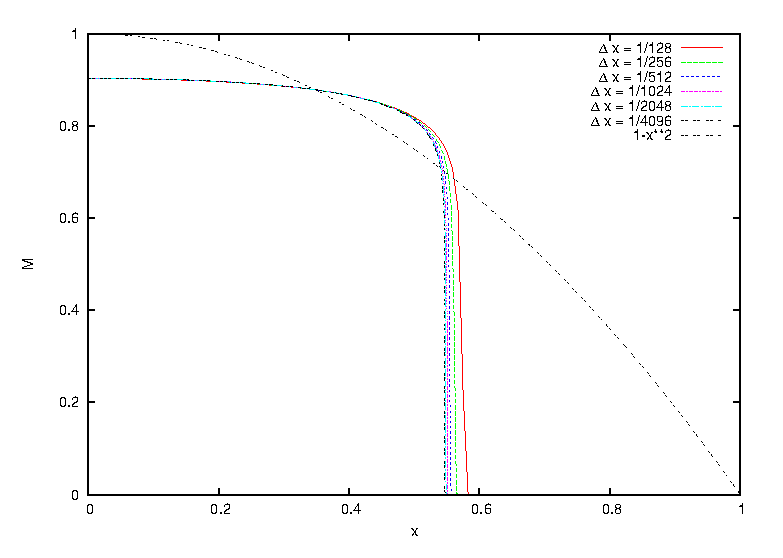
\includegraphics[scale=0.55]{Cfunc_polynomial_t=5-25.eps} &
          \includegraphics[scale=0.55]{Cfunc_polynomial_interface.eps} \\
          (a) & (b) 
      \end{tabular}
      \caption{Convergence of solutions for $\hat{C}(x) = 1-x^2$ looking at (a) solutions at $t = 5.25$ and (b) the interface x position.}
      \label{fig:functionC}
    \end{center}
  \end{figure}
  
   Figure \ref{fig:kinematics} show how the solutions converge for different functions $f(C,M)$. Some of which do not depend on $C$ or $M$. 
  
  \begin{figure}[h!tb]
    \begin{center}
      \begin{tabular}{c c}
          \includegraphics[scale=0.55]{Fdefault.eps} &
          \includegraphics[scale=0.55]{FdefaultInterface.eps} \\
          (a) & (b) \\
          \includegraphics[scale=0.55]{Flogistic_t=4-25.eps} &
          \includegraphics[scale=0.55]{Flogistic.eps} \\
          (c) & (d) \\
          \includegraphics[scale=0.55]{FnoM.eps} &
          \includegraphics[scale=0.55]{FnoMInterface.eps} \\
          (e) & (f) \\
          \includegraphics[scale=0.55]{Fconstant.eps} & \\
          (g) & \\ 
      \end{tabular}
      \caption{Convergence of solutions for (a-b) $f(C,M) = $default,  (c-d) $f(C,M) = (1 - M)$, (e-f) $f(C,M) = (1 - C) \frac{C}{M+\epsilon}, $(g) $f(C,M) = 1$. Each pair of graphs is the solution at $t = 4.25$ and the interface as a function of t.}
      \label{fig:kinematics}
    \end{center}
  \end{figure}



\chapter{Simulation Results}
\section{Typical Simulation}
Is Typical\_simulation.tex needed in this section?
If anything it would be the sanity check simulations


The system
  \begin{align}
    M_t &= \nabla_x \left( D(M) \nabla_x M \right) + f(C,M) M \\
    C_t &= - g(C,M) 
  \end{align}
  where
  \begin{align}
    D(M) &= \delta \frac{M^\alpha}{(1 - M)^\beta} \\
    f(C,M) &= \frac{ C }{{k } + {C}} \left(1 - \left( \frac{M M_0}{{C C_0 + \epsilon}} \right)^\gamma \right) \\
    g(C,M) &= \frac{\nu C}{k +C} M
  \end{align}
  is solved on a rectangular region with length $L$ and width $\lambda L$ with the following parameter values,
  \begin{equation}
    \begin{aligned}
      L &= 0.01 \\
      \lambda &= \frac{1}{128}\\
      \epsilon &= 10^{-8}\\
      \alpha &= 4 \\
      \beta &= 4 \\
      \gamma &= 0.5 \\
      \mu &= 6 \\      
    \end{aligned}
    \qquad
    \begin{aligned}
      C_0 &= 30 \\
      M_0 &= 30 \\
      \delta &= \frac{10^{-7}}{\mu L^2} \approx 10^-4\\
      k &= \frac{4}{C_0} \approx 0.1333\\
      \nu &= \frac{M_0}{0.63 C_0} \approx 1.59,\\
    \end{aligned}
  \end{equation}
  and with initial conditions 
  \begin{equation}
    \begin{aligned}
      C &= 1 \\
      M &= \begin{cases} -(\frac{h}{d^4})x^4 + h & \text{if } x < 0.04 \\ 0 & \text{otherwise }\end{cases} \\
    \end{aligned}
  \end{equation}  
  where $h = 0.05, d=0.04$ , representing the height and depth of the inoculation site.

  A series of test was done on simulation code version $0.1.1$. These were defaulted to run with $\Delta t = 10^{-3}$ and $\Delta x = \frac{1}{256}$.
  
  The following lists the test, and observations from each.
  
  \begin{enumerate}
    \item Solve the system with homogenous initial conditions and see if it stays homogenous.
      \begin{itemize}
        \item Worked!
        \item The biomass and substrate concentration at $t=8$ did not change as grid size did, which is good. 
        \item Biomass and substrate concentration did change for step size, but it was converging to a specific value (Table \ref{tab:homoIC}), which makes sense and suggests that default choice of $\Delta t$ is good.
        \begin{table}
          \begin{center}
            \begin{tabular}{| c | c | c |}
              \hline
              $\Delta t$ & Biomass Density & Substrait Conc. \\
              \hline
              $10^{-1}$ & 0.743806469443 & 0.731575100108\\
              $10^{-2}$ & 0.739180637812 & 0.736539504220\\
              $10^{-3}$ & 0.738699851204 & 0.737025027162 \\
              $10^{-4}$ & 0.738651598939 & 0.737073472750\\
              $10^{-5}$ & 0.738646771985 & 0.737078316244\\
              \hline
            \end{tabular}
            \caption{Values of biomass and substrate concentration at $t = 8$. A grid size of $\Delta x = 1/256$ was used.}
            \label{tab:homoIC}
          \end{center}
        \end{table}
      \end{itemize}

%    \item Solve the system with non-homogenous high initial condition ($M_0=0.95$), with zero forcing term, and see if density-dependent diffusion moves it without loss of biomass.
%      \begin{itemize}
%        \item DOESN"T WORK!!!!!!
%      \end{itemize}
  
      
    \item Solve the system with $f = s$, $s$ a constant, and see if total biomass follows $be^{st}$, where $b$ is the initial total biomass.
    \begin{itemize}
      \item Works with $D(M) = 0$.
      
      \item With $D(M) = \delta$ total biomass grows a little slower then $be^{st}$ which becomes slightly noticable at later times. The difference is less then 1\%, so this looks good. See Figure \ref{fig:totalBioCheck}(ab).
      
      \item With $D(M) = \delta M^{\alpha}$ the total biomass matchs $be^{st}$ until the biomass density at the innoculation point becomes greater then 1. Since physically this should never occur, this isn't a problem.  See Figure \ref{fig:totalBioCheck}(c).
      
      \item With $D(M) = \frac{\delta M^{\alpha}}{(1-M)^\beta}$ the total biomass grows accuratly until it approches $M \in (0.9, 1)$ at the innoculation point. This is a problem, because at this point the density dependent diffusion should start and keep the solution growing with $be^{st}$. This suggests that there is something wrong with how the diffusion is being implemented, will follow up on this.  See Figure \ref{fig:totalBioCheck}(d).
      
      \begin{figure}
        \begin{center}
          \begin{tabular}{c c}
            \includegraphics[scale=0.5]{checkTotal_Dconstant.eps} &
            \includegraphics[scale=0.5]{checkTotal_Dconstant_zoomed.eps} \\
            (a) & (b) \\
            \includegraphics[scale=0.5]{checkTotal_Dporous.eps} & 
            \includegraphics[scale=0.5]{checkTotal_Ddensity.eps} \\
            (c) & (d) \\
          \end{tabular}
          \captionsetup{singlelinecheck=off}
          \caption[enum]{Graph of, 
            \begin{enumerate}[(a)]
              \item $D(M) = \delta$, 
              \item $D(M) = \delta$; zoomed in to show the slight difference in growth,
              \item $D(M) = \delta M^\alpha$,
              \item $D(M) = \frac{\delta M^{\alpha}}{(1-M)^\beta} $.
            \end{enumerate} 
          }

          \label{fig:totalBioCheck}
        \end{center}
      \end{figure}
      
    \end{itemize}
      
  \end{enumerate}

\chapter{Discussions}
Lots of discussion on the things that were analysied in this thesis.

\chapter{Conclusions}
There will be lots of concluding statements in here.


\newpage
\pagestyle{References}
\chapter*{References}
\addcontentsline{toc}{chapter}{\hspace{16pt} Complete Bibliography}
\titlespacing{\section}{0pt}{*0}{*0}
\renewcommand{\bibname}{}
\renewcommand\bibsection{}
\titlespacing{\chapter}{0pt}{*0}{*0}
\titlespacing{\section}{0pt}{*0}{*0}
\setlength{\parskip}{0pt}
\setlength{\parsep}{0pt}
\nocite*
\bibliographystyle{plainnat}
\bibliography{ThesisReferences}



\newpage
\pagestyle{fancy}

%%Appendix A Behavioural Plots Simulation Study
%\input{BackMatter/AppendixA}


\newpage
\thispagestyle{custom}
\mbox{}


\end{document}
